\documentclass{beamer}
%
% Choose how your presentation looks.
%
% For more themes, color themes and font themes, see:
% http://deic.uab.es/~iblanes/beamer_gallery/index_by_theme.html
%
\mode<presentation>
{
  \usetheme{default}      % or try Darmstadt, Madrid, Warsaw, ...
  \usecolortheme{default}
  \usepackage{beamerthemesplit}% or try albatross, beaver, crane, ...
  \usefonttheme{default}  % or try serif, structurebold, ...
  \setbeamertemplate{navigation symbols}{}
  \setbeamertemplate{caption}[numbered]
  \usepackage{circuitikz}
  \usepackage{tikz}
} 

\usepackage[english]{babel}
\usepackage[utf8x]{inputenc}
\usepackage{amsmath}

% \logo{\vspace{-0.3cm}\includegraphics[height=0.75cm]{D0.png}}
\title[ \hspace{0.5cm}\insertframenumber/\inserttotalframenumber]{Attention Is All You Need}
\author{Shah Jainam EE21B122 \& Ayush Ranjan EE21B026}
\institute{Indian Institute of Technology \\ Madras}
\date{25-04-2025}

\begin{document}

\begin{frame}
  \titlepage
\end{frame}

% Uncomment these lines for an automatically generated outline.
%\begin{frame}{Outline}
%  \tableofcontents
%\end{frame}

%\section{Introduction}

\begin{frame}{Machine Translation Problem}

\begin{itemize}
    \item The motivation for this paper is to solve the problem of text translation.
    \item  Recurrent neural networks, long short-term memory \footnote{Sepp Hochreiter and Jürgen Schmidhuber,1997} and gated recurrent \footnote{Junyoung Chung, Çaglar Gülçehre, Kyunghyun Cho, and Yoshua Bengio} neural networks in particular, have been firmly established as state of the art approaches in sequence modeling and transduction problems such as language modeling and machine translation
\end{itemize}

\begin{figure}[htbp]
    \centering
    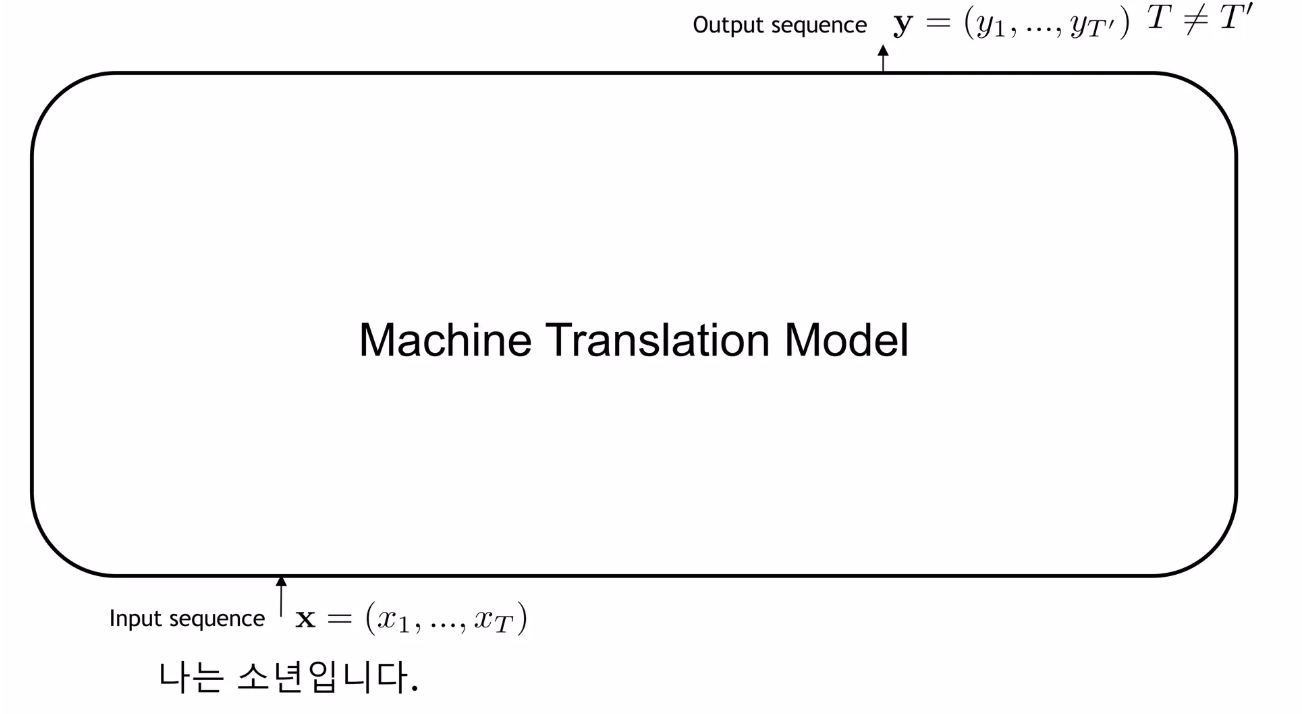
\includegraphics[width=0.6\linewidth]{f1.png}
    \label{fig:enter-label}
\end{figure}
\end{frame}

\begin{frame}{RNN Encoder-Decoder Model}
\begin{figure}
    \centering
    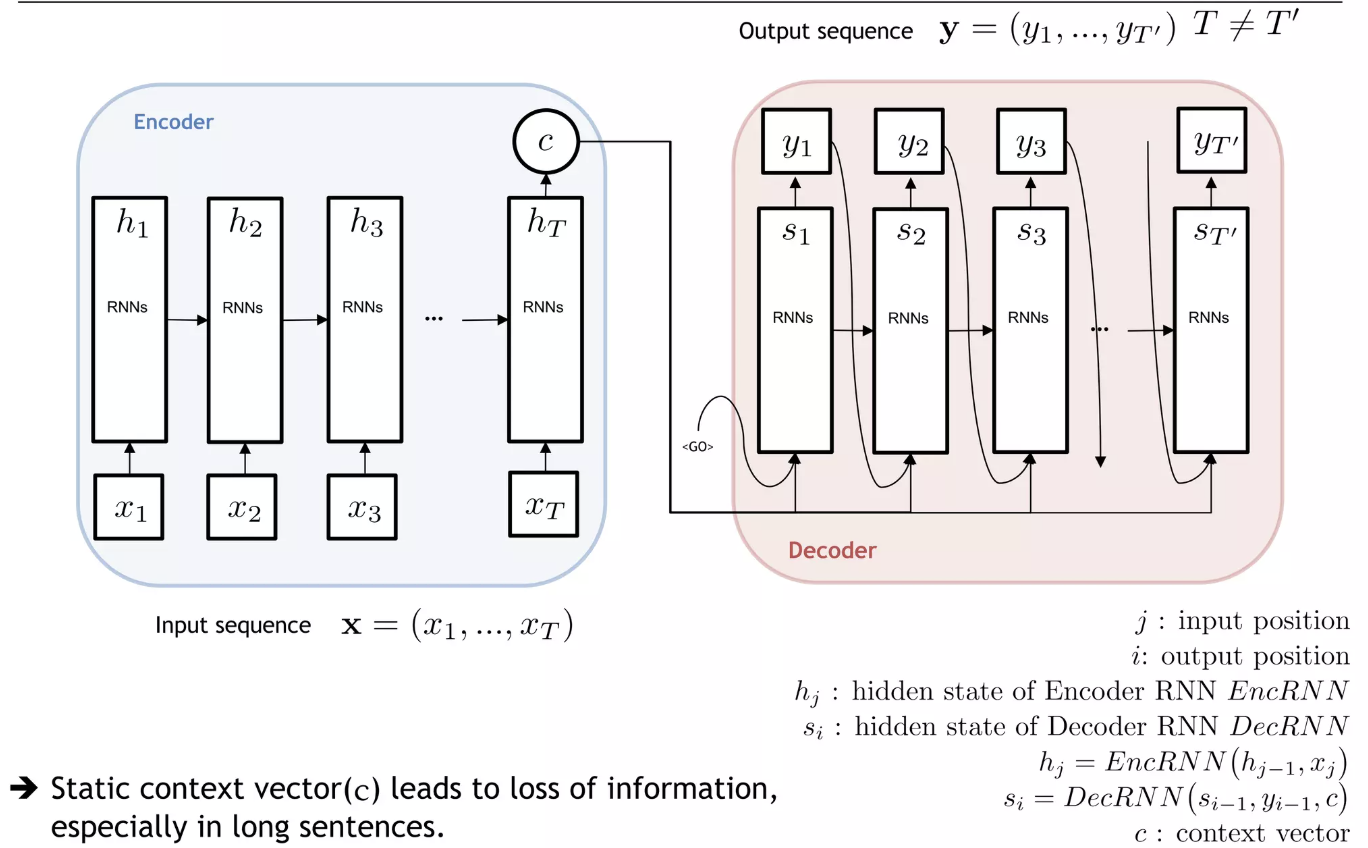
\includegraphics[width=1\linewidth]{f2.png}
    \label{fig:enter-label}
\end{figure}
    
\end{frame}

\begin{frame}{Limits of Recurrent Neural Network}

\begin{itemize}
    \item RNN generates each hidden state in series.
        \begin{itemize}
            \item This sequential nature increases the training time by a large margin.
        \end{itemize}
    \item RNN has long term dependency problems.
        \begin{itemize}
            \item It's hard to remember long term context information.
            \item Attempts to add attention mechanism to RNN have been tried. \footnote{Neural Machine Translation by Jointly Learning to Align and Translate Dzmitry Bahdanau, Kyunghyun Cho, Yoshua Bengio}
        \end{itemize}
    \item RNN can see one word at a time
        \begin{itemize}
            \item CNN can see more than one at a time.
        \end{itemize}
\end{itemize}
\end{frame}

\begin{frame}{Transformers}
\begin{itemize}
    \item Transformers were developed to solve the problem of machine translation and sequence transduction, or neural machine translation, but they can do so much more.
\end{itemize}

\begin{columns}
  % Left Column for Image
  \column{0.4\textwidth}
  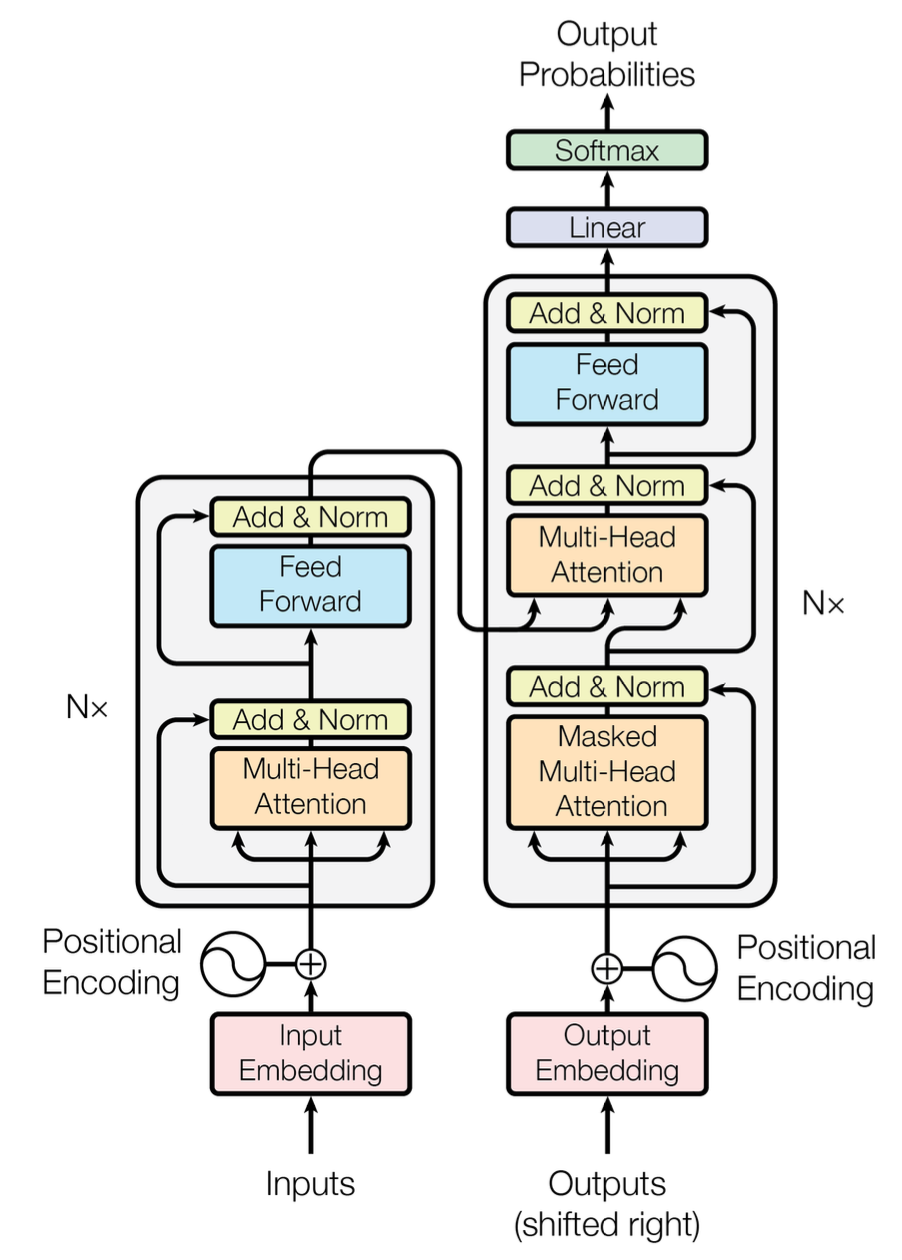
\includegraphics[width=1\linewidth]{f3.png} % Replace with your image filename

  % Right Column for Text
  \column{0.6\textwidth}
      \begin{itemize}
          \item Great performance in computer vision like ViT (Dosovitskiy, 2020)
          \item Image Classification (CoCa Transformer)
          \item Semantic Segmentation (e.g., FD-SwinV2-GTransformer)
          \item Object Detection (e.g., FD-SwinV2-GTransformer)
      \end{itemize}

\end{columns}
\end{frame}

\begin{frame}{Full Architecture of Transformer.}
    \begin{figure}
        \centering
        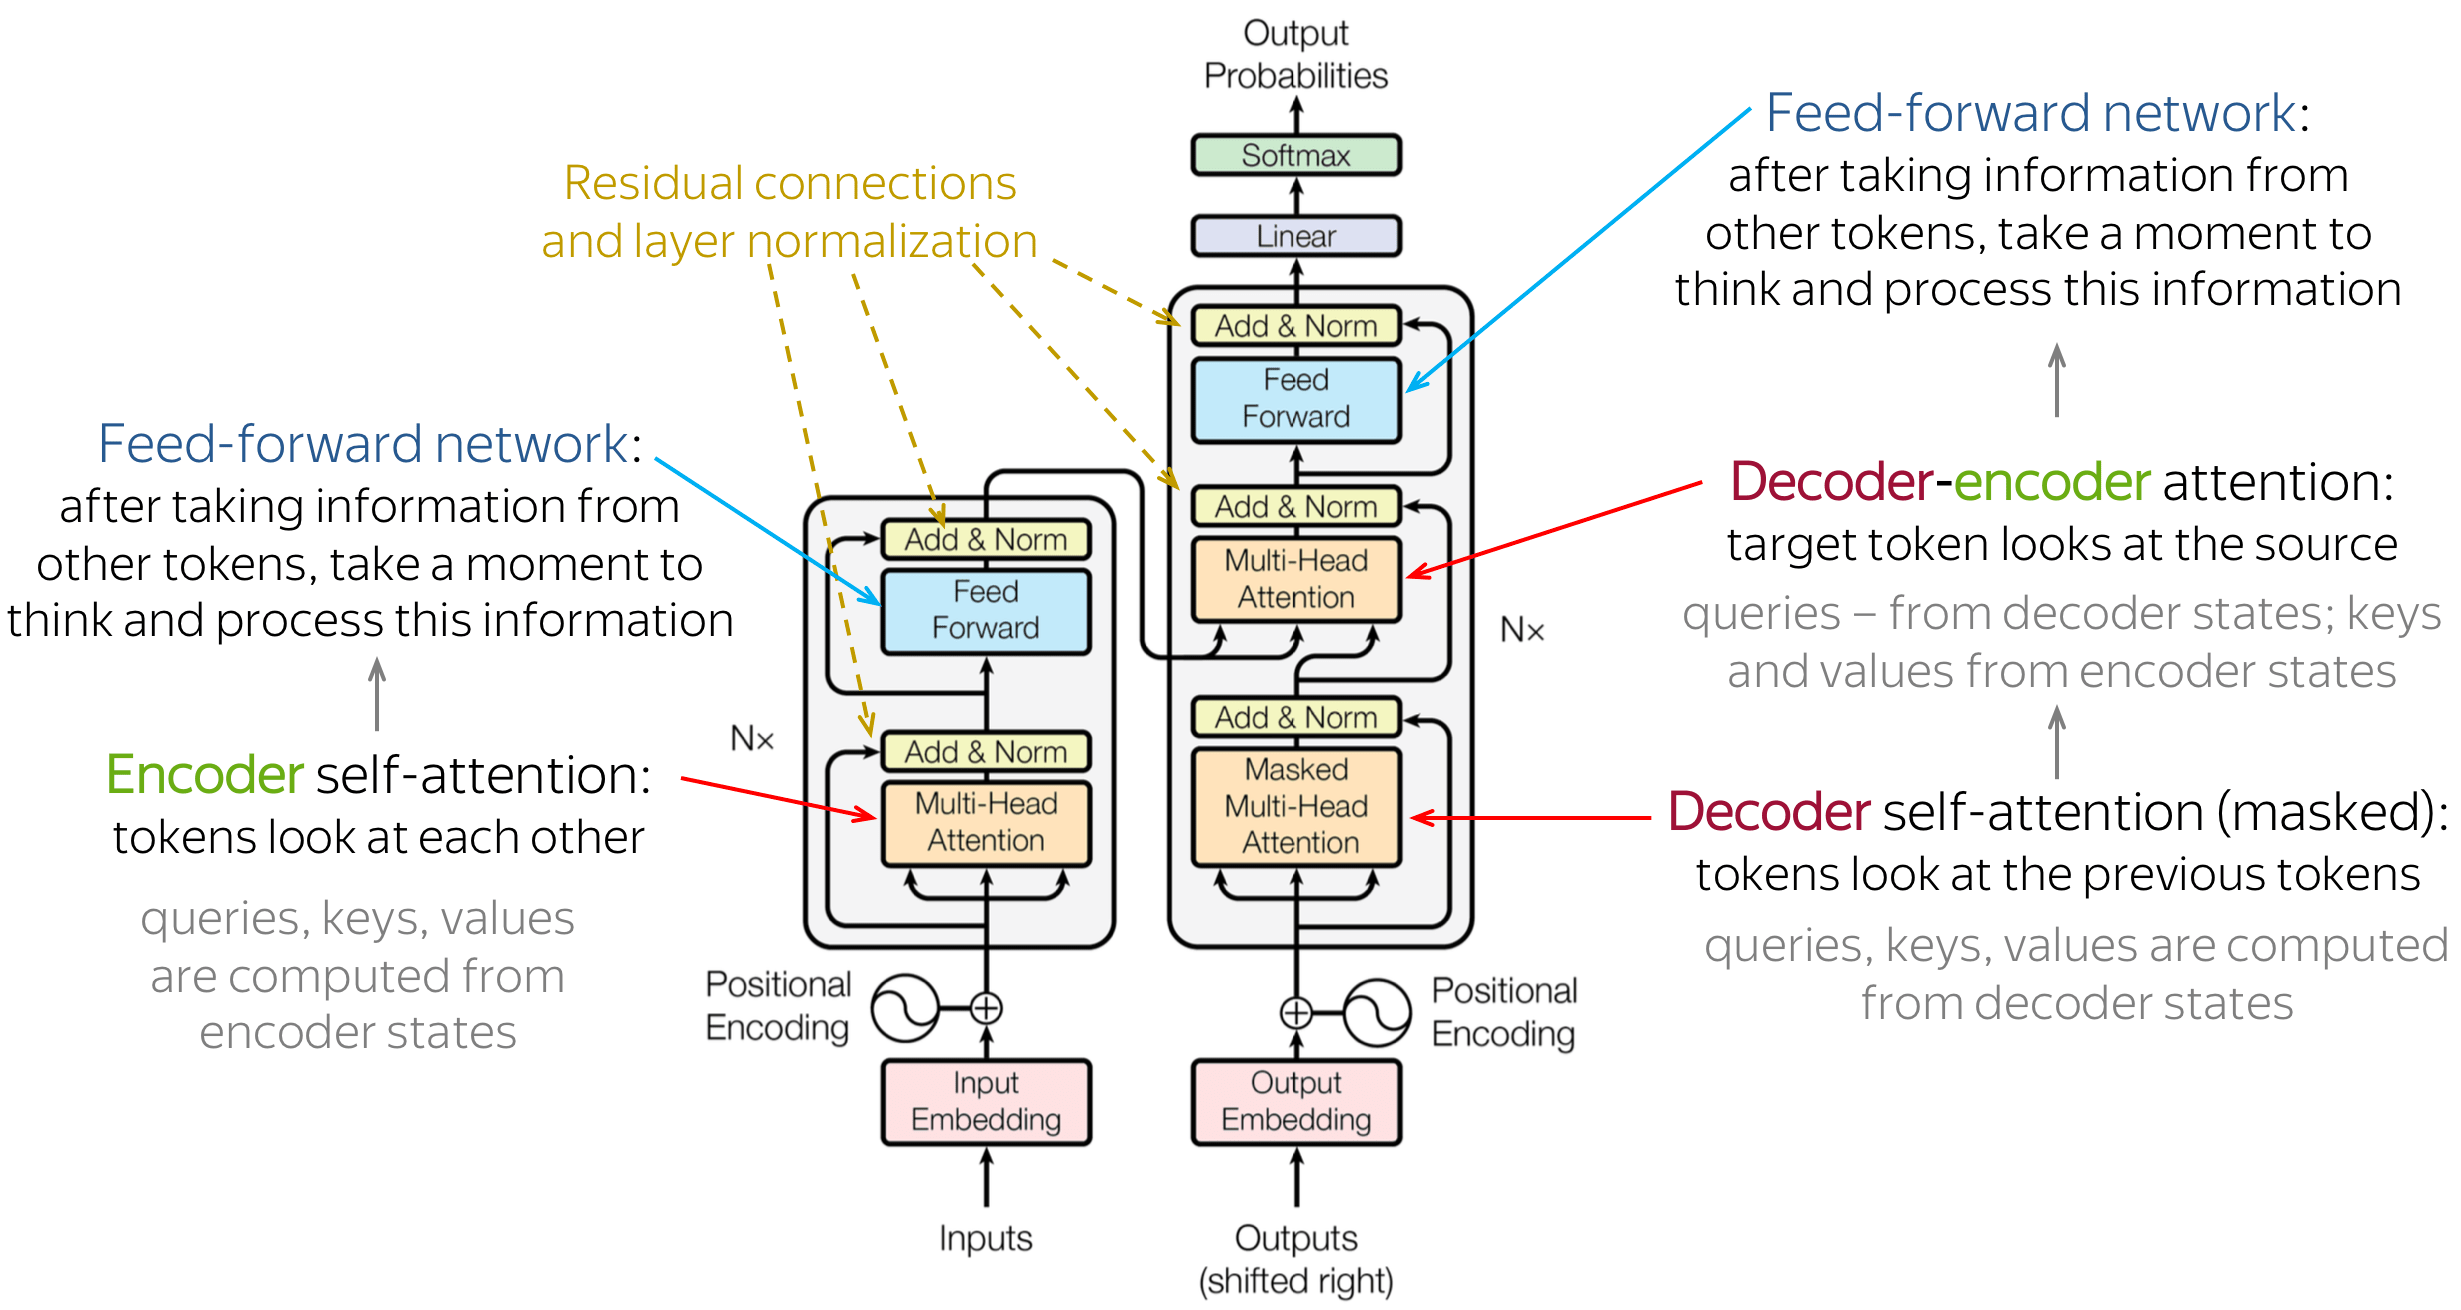
\includegraphics[width=1\linewidth]{f4.png}
        \label{fig:enter-label}
    \end{figure}
    \renewcommand{\thefootnote}{}
\footnotetext{image credits: Lena Voita}
\renewcommand{\thefootnote}{\arabic{footnote}}

\end{frame}

\begin{frame}{Encoder Architecture}
\begin{itemize}
    \item Encoder is made up of 6 identical layers
\end{itemize}
\begin{columns}

  \column{0.25\textwidth}
  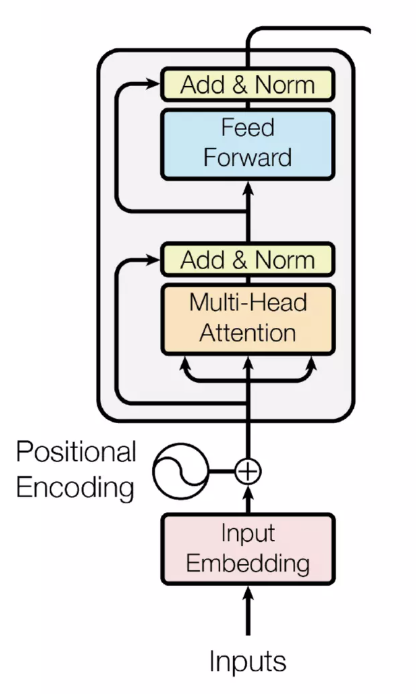
\includegraphics[width=1\linewidth]{f5.png} % Replace with your image filename
  \column{0.75\textwidth}
\begin{itemize}

    \item Each layer has two sub-layers. 
        \begin{itemize}
            \item  First is multi-head self-attention mechanism, 
            \item Second is a simple, position- wise fully connected feed-forward network.
        \end{itemize}
    \item Residual connections\footnote{Kaiming He, Xiangyu Zhang, Shaoqing Ren, and Jian Sun,2016} + Layer Normalizations\footnote{Jimmy Lei Ba, Jamie Ryan Kiros, and Geoffrey E Hinton,2016}.
    \texttt{LayerNorm(x+Sublayer(x))}
    \item To facilitate these residual connections, all sub-layers in the model, as well as the embedding layers, produce outputs of dimension $d_{model} = 512.$
\end{itemize}  
\end{columns}  
\end{frame}

\begin{frame}{Decoder Architecture}

\begin{columns}
  \column{0.25\textwidth}
  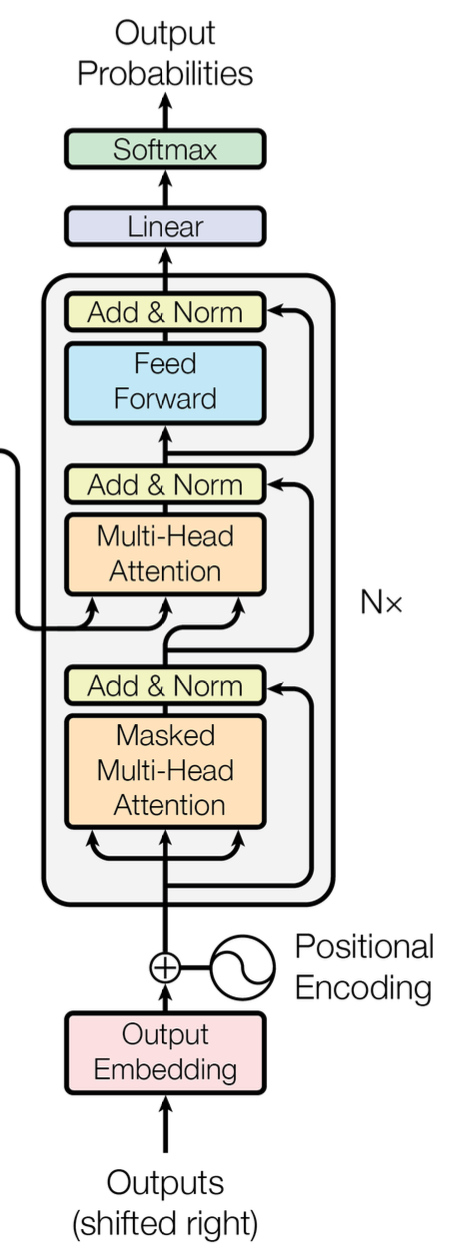
\includegraphics[width=1\linewidth]{f6.png} % Replace with your image filename

  \column{0.75\textwidth}
  \begin{itemize}
      \item The decoder is also composed of a stack of N = 6 identical layers.
      \item In addition to the two sub-layers in each encoder layer, the decoder inserts a third sub-layer, which performs multi-head attention over the output of the encoder stack.
      \item Also modify the self-attention sub-layer in the decoder stack to prevent positions from attending to subsequent positions. 

  \end{itemize}
\end{columns}
\end{frame}

\begin{frame}{Embedding and Positional Encoding.}

\begin{columns}
  \column{0.3\textwidth}
  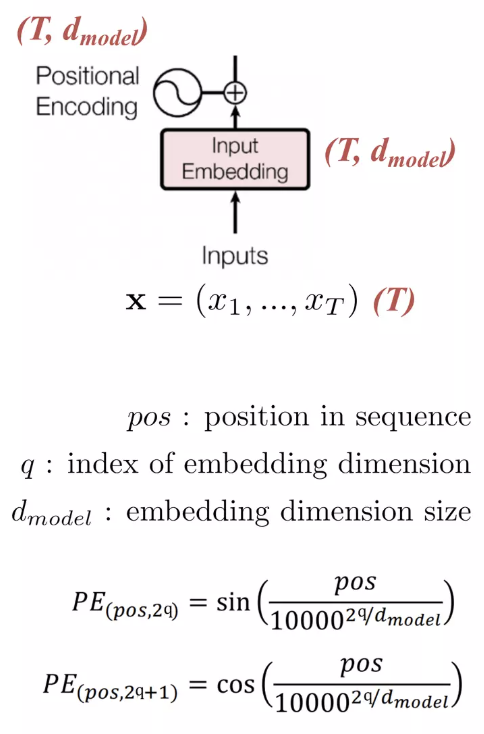
\includegraphics[width=1.25\linewidth]{f7.png} % Replace with your image filename
  \column{0.7\textwidth}
  \begin{itemize}
    \item Transformer does not contain recurrence or convolution, it does not know the order of input tokens.
    \item For this, there are two sets of embeddings: for tokens and for positions(different from rnn).
    \item Then input representation of a token is the sum of two embeddings(both of dimension $d_{model}$)\footnote{Jonas Gehring, Michael Auli, David Grangier, Denis Yarats, and Yann N. Dauphin, 2017.
}
    \item  Each dimension of the positional encoding corresponds to a sinusoid and form a geometric progression from $2\pi$ to $10000\pi$
\end{itemize}
\end{columns}
\end{frame}

\begin{frame}{Attention}
    \begin{itemize}
        \item An attention function can be described as mapping a query and a set of key-value pairs to an output, where the query, keys, values, and output are all vectors. 
        \item The output is computed as a weighted sum of the values, where the weight assigned to each value is computed by a compatibility function of the query with the corresponding key.
        \item The input consists of queries and keys of dimension $d_k$ , and values of dimension $d_v$, divide each by $\sqrt{d_k}$, and apply a softmax function to obtain the weights on the values.
    \end{itemize}
    
    \vspace{0.5em}
    \begin{columns}
        % Left column for formula
        \column{0.45\textwidth}
        \[
        \text{Attention}(Q, K, V) = \text{softmax}\left(\frac{QK^T}{\sqrt{d_k}}\right)V
        \]

        % Right column for image
        \column{0.05\textwidth}
        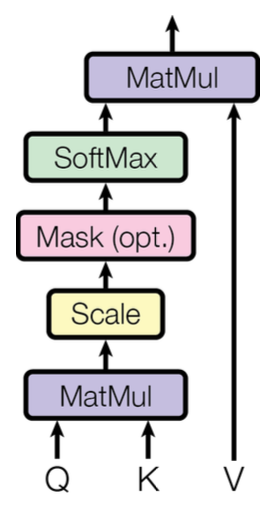
\includegraphics[width=3\linewidth]{f8.png} % Adjust image width if needed
    \end{columns}
\end{frame}

\begin{frame}{Idea behind the Attention}
\begin{columns}
  \column{0.4\textwidth}
  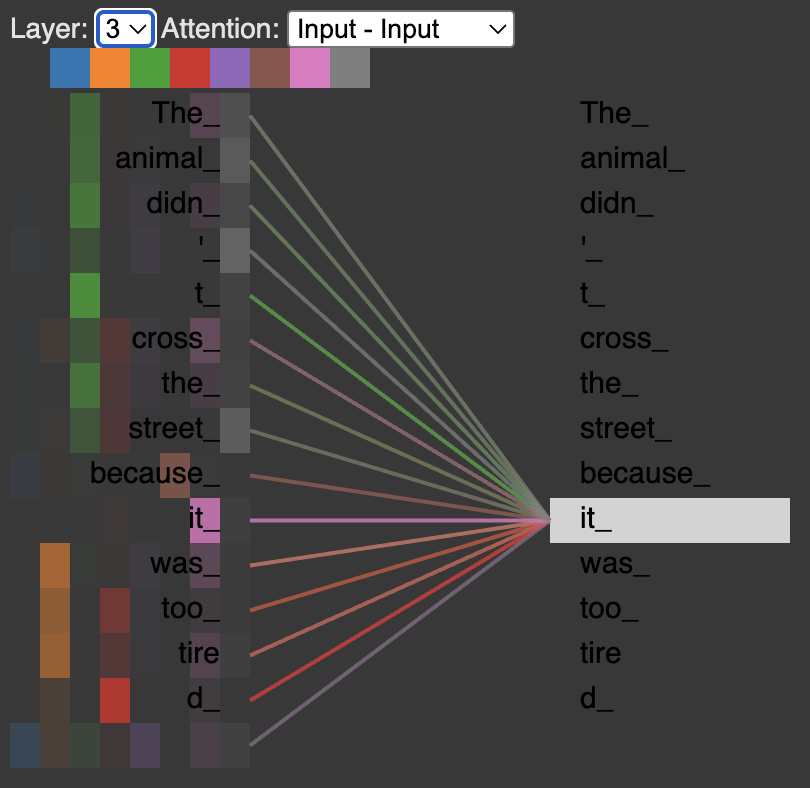
\includegraphics[width=1\linewidth]{f12.png}
  \column{0.6\textwidth}
  \begin{itemize}
      \item Each element attends to every other element
      \item It is an attention mechanism relating different positions of a single sequence in order to compute a representation of the same sequence
      \item Each element becomes query, key, and value from the input embeddings by multiplying by a weight matrix
  \end{itemize}
    
\end{columns}
\renewcommand{\thefootnote}{}
\footnotetext{https://github.com/tensorflow/tensor2tensor}
\renewcommand{\thefootnote}{\arabic{footnote}}

\end{frame}

\begin{frame}{Maths behind Attention}

\begin{itemize}
    \item Learn (differentiable) how to pick relevant information from input data.
\end{itemize}

\begin{columns}
    \column{0.4\textwidth}
        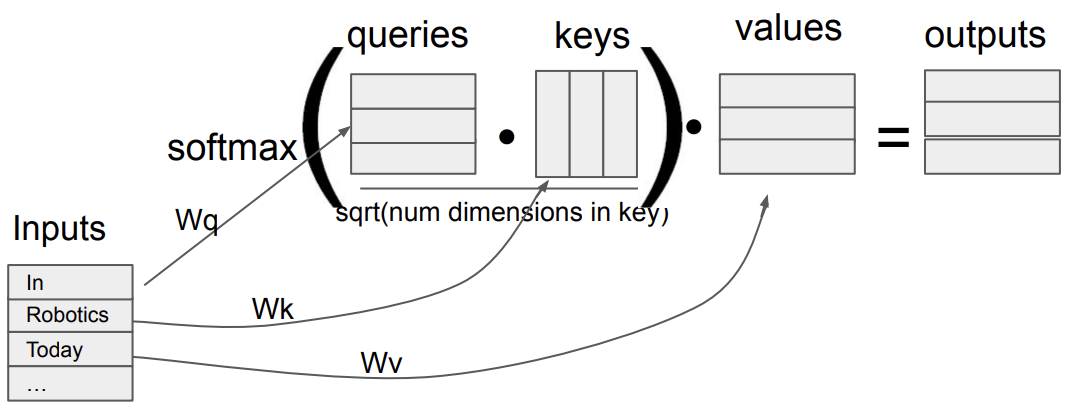
\includegraphics[width=1.2\linewidth]{f9.png} 

    \column{0.6\linewidth}
      \begin{itemize}
        \item Create three vectors from each of the encoder’s input value (query, key, value)
        \item Calculate a score for how much to focus on each part of the input when we encode words at specific positions
        \item Dividing by $d_k$ makes algorithm easier to train
      \end{itemize}
    \end{columns}

\begin{itemize}
    \item The idea is to select a value (referenced by a key) relevant to a query (what trying to pull from input)
\end{itemize}

\end{frame}


\begin{frame}{Scaled-Dot Product Attention}

$d_{model}$ : embedding or attention dimentions(=512)

$T$: Input sequence length

$Q,K,V \in \Re^{T \texttt{x} d_{model}}$

\begin{columns}
  \column{0.2\textwidth}
  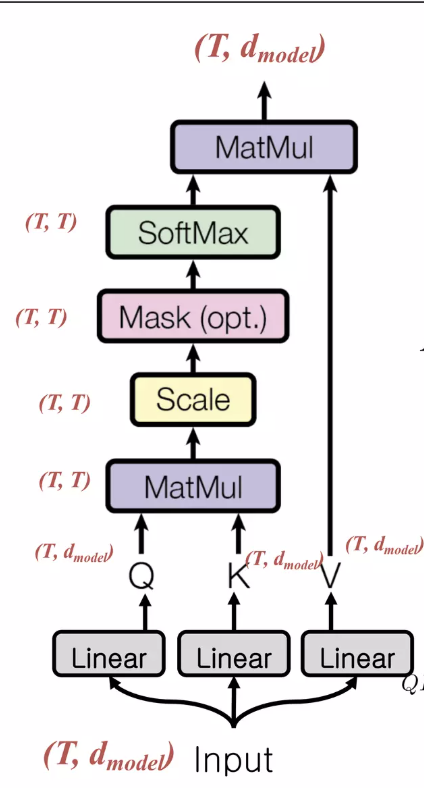
\includegraphics[width=1.25\linewidth]{f11.png} % Replace with your image filename

\column{0.8\textwidth}


        $
        \text{Attention}(Q, K, V) = \text{softmax}\left(\frac{QK^T}{\sqrt{d_k}}\right)V
        $




\begin{columns}

\column{0.4\textwidth}
$
V = \Bigg[
\begin{array}{ccc}
- & v_{1}^T & - \\
- & v_{2}^T & -  \\
\vdots & \vdots & \vdots \\
- & v_{T}^T & -
\end{array}
\Bigg]_{T \texttt{x} d_{model}}
$
\column{0.6\textwidth} 
$
QK^T = \Bigg[
\begin{array}{cccc}
a_{11} & a_{12} & \cdots & a_{1T} \\
a_{21} & a_{22} & \cdots & a_{2T} \\
\vdots & \vdots & \ddots & \vdots \\
a_{T1} & a_{T2} & \cdots & a_{TT}
\end{array}
\Bigg]_{T\texttt{x}T}
$

\end{columns}


$
QK^TV = \Bigg[
\begin{array}{ccc}
- & \Sigma_{k=1}^Ta_{1k}v_{k}^T & - \\
- & \Sigma_{k=1}^Ta_{2k}v_{k}^T & -  \\
\vdots & \vdots & \vdots \\
- & \Sigma_{k=1}^Ta_{Tk}v_{k}^T & -
\end{array}
\Bigg]_{T \texttt{x} d_{model}}
$




\end{columns}

    
\end{frame}








\begin{frame}{Attention continue...}

% \begin{itemize}
%     \item The main idea that a network can learn which input parts are more important at each step. Since everything here is differentiable (attention function, softmax, and all the rest), a model with attention can be trained end-to-end. We don't need to specifically teach the model to pick the words you want - the model itself will learn to pick important information.
% \end{itemize}
The general computation scheme is shown below.\renewcommand{\thefootnote}{}
\footnotetext{image credit: Lena Voita}
\renewcommand{\thefootnote}{\arabic{footnote}}


\begin{figure}
    \centering
    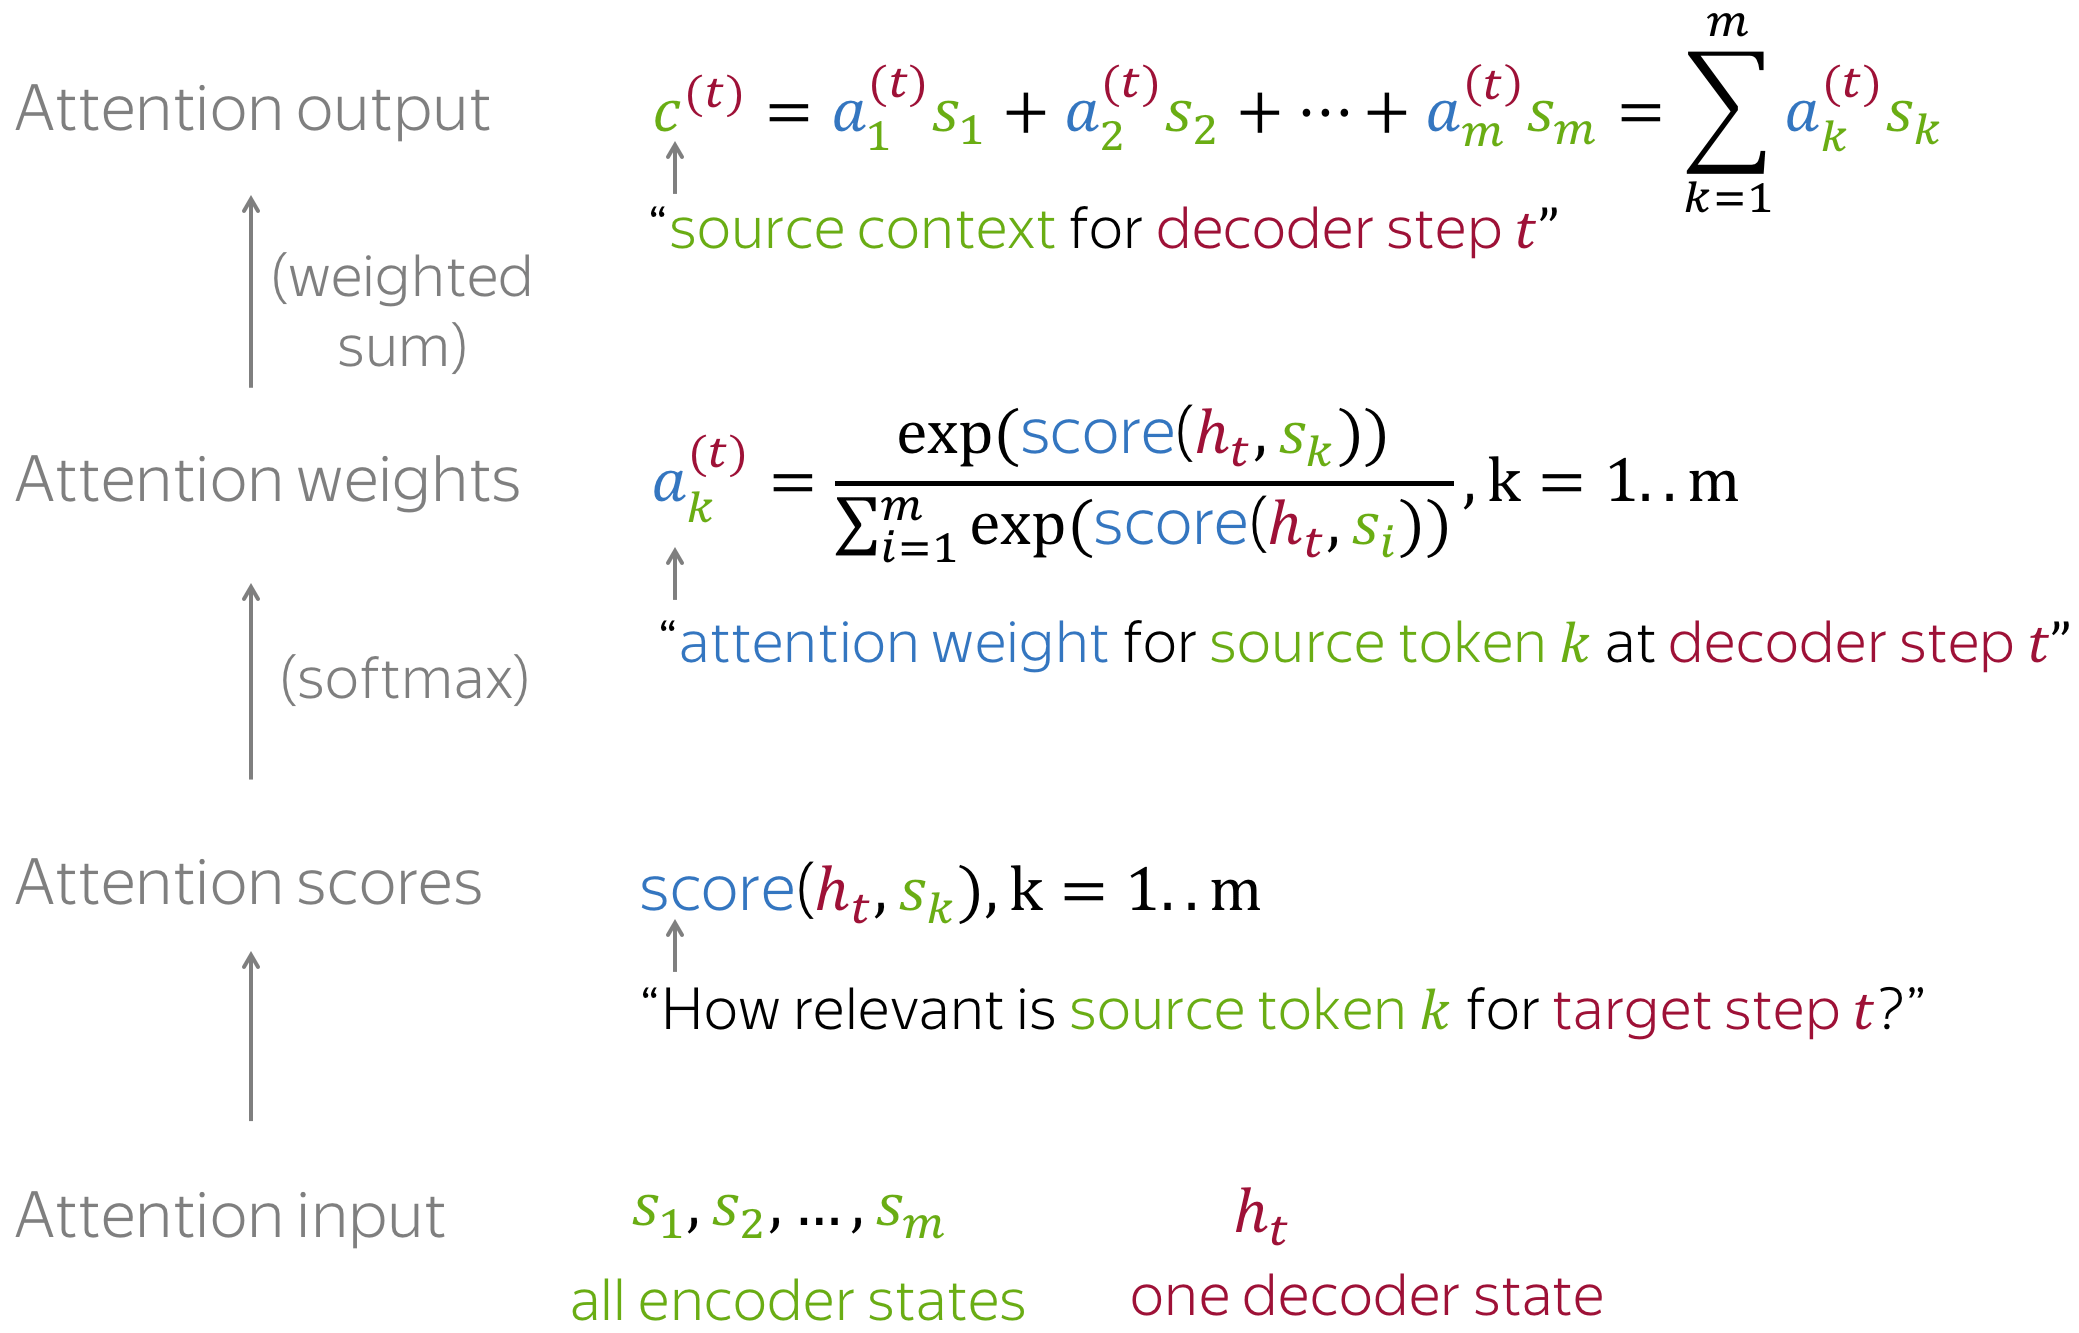
\includegraphics[width=0.8\linewidth]{f10.png}
    \label{fig:enter-label}
\end{figure}
    
\end{frame}

\begin{frame}{Multi-Head Attention}

\begin{itemize}
  \item Queries, keys, and values are \textbf{linearly projected} $h$ times using \textbf{different learned linear projections} into smaller dimensions ($d_k$, $d_v$).
  
  \item Attention is applied \textbf{independently} to each set of projected vectors in parallel, producing multiple $d_v$-dimensional outputs.
  
  \item The outputs from all heads are \textbf{concatenated} and passed through a final linear layer to produce the output.
  
  \item Multi-head attention allows the model to \textbf{attend to information from different subspaces and positions simultaneously}, improving representational capacity.
  \begin{align*}
    \text{MultiHead}(Q, K, V) &= \text{Concat}(\text{head}_1, ..., \text{head}_h)W^O \\
    \text{where} \quad \text{head}_i &= \text{Attention}(QW^Q_i, KW^K_i, VW^V_i)
  \end{align*}

  \item Using multiple heads with reduced dimensions (e.g., $d_k = d_v = \frac{d_{\text{model}}}{h} = 64$, $h = 8$) \textbf{keeps computational cost similar} to single-head attention.
\end{itemize}
    
\end{frame}

\begin{frame}{Why multi-head attention...}

\begin{itemize}
    \item Allows for model to focus on different positions
    \item Gives attention layer multiple “representation subspaces”
    \item No longer need to oversaturate one attention mechanism
\end{itemize}

\begin{columns}
  \column{0.3\textwidth}
  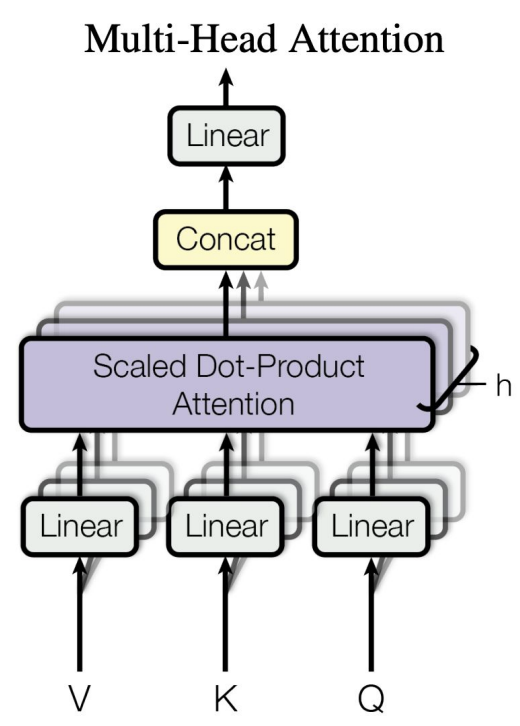
\includegraphics[width=1\linewidth]{f14.png} % Replace with your image filename

  \column{0.7\textwidth}
  \textbf{Learned Parameters:}
  \begin{align*}
    W^Q_i &\in \mathbb{R}^{d_{\text{model}} \times d_k} \\
    W^K_i &\in \mathbb{R}^{d_{\text{model}} \times d_k} \\
    W^V_i &\in \mathbb{R}^{d_{\text{model}} \times d_v} \\
    W^O   &\in \mathbb{R}^{h \cdot d_v \times d_{\text{model}}}
  \end{align*}
\end{columns}

Using multiple heads with reduced dimensions (e.g., $d_k = d_v = \frac{d_{\text{model}}}{h} = 64$, $h = 8$) \textbf{keeps computational cost similar} to single-head attention.
    
\end{frame}

\begin{frame}{Zoom into Encoder}\renewcommand{\thefootnote}{}
\footnotetext{editing credit: Shah Jainam}
\renewcommand{\thefootnote}{\arabic{footnote}}
\begin{figure} 
    \centering
    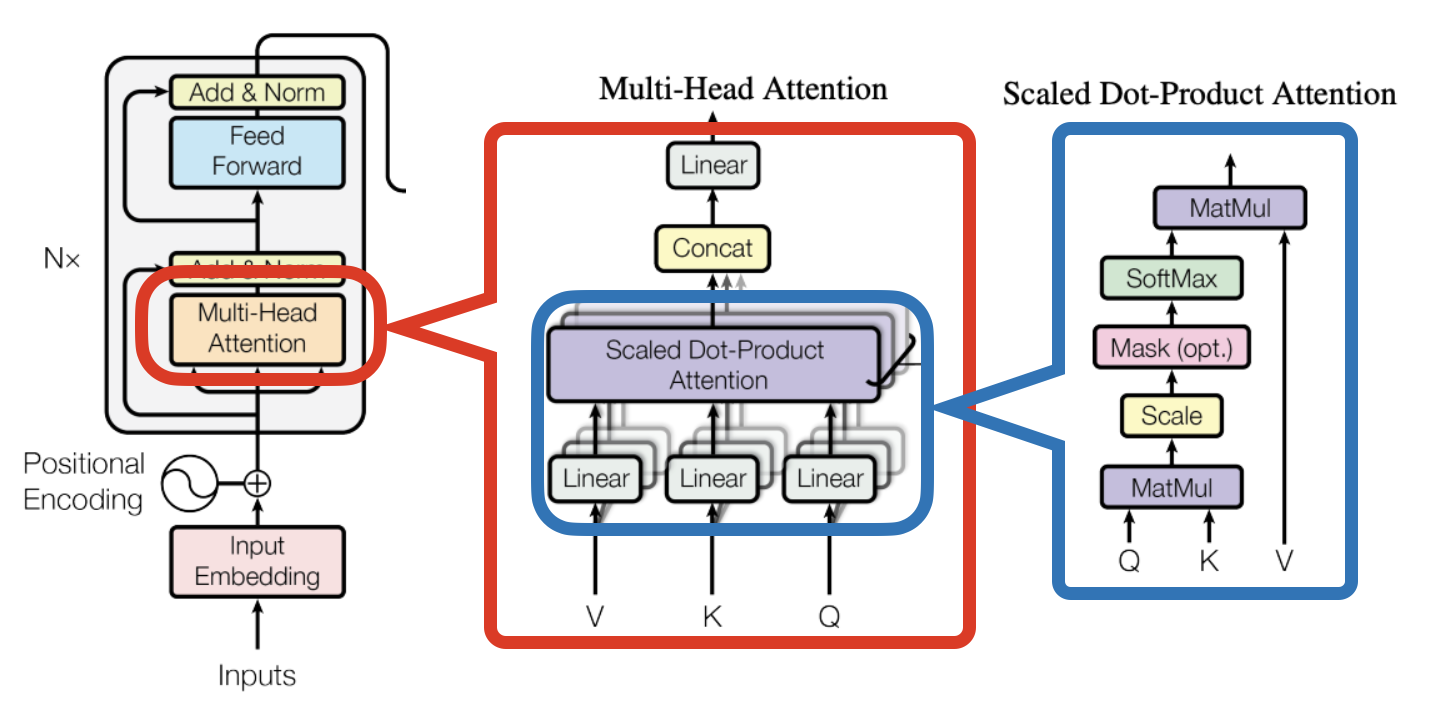
\includegraphics[width=1\linewidth]{f15.png}
    \label{fig:enter-label}
\end{figure}
\end{frame}

\begin{frame}{Masked Attention}

\begin{itemize}
    \item Masking hides future tokens during each prediction.
    \item Prevents the model from "cheating" by seeing future outputs.
    \item It also allows the model to train in parallelization.
\end{itemize}

\begin{columns}

  \column{0.5\textwidth}
  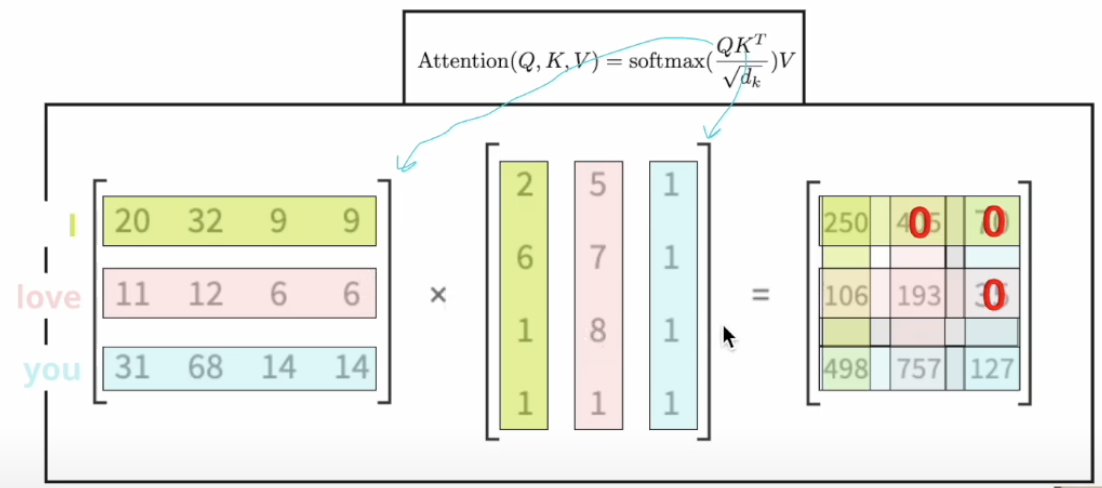
\includegraphics[width=1\linewidth]{f16.png}\renewcommand{\thefootnote}{}
\footnotetext{image credit: Deep Study(Youtube Channel)}
  \column{0.5\textwidth}

  \begin{itemize}
      \item   The training algorithm knows the entire expected output. It hides (masks) a part of this known output sequence for each of the parallel operations.
  \end{itemize}    
\end{columns}

\begin{itemize}
    \item During inference, the decoder works sequentially, generating one token at a time since the full output is unknown.
    \item The model learns to predict masked words using context from the visible (non-masked) words.
\end{itemize}

\end{frame}

\begin{frame}{Cross Attention}

\begin{itemize}
    \item  Cross-attention acts as a bridge between the encoder and decoder. It allows the decoder to "ask" the encoder which parts of the input are most relevant for decoding.
\end{itemize}


\begin{columns}
    \column{0.35\linewidth}
        \vspace{2em} % Adjust this value as needed
        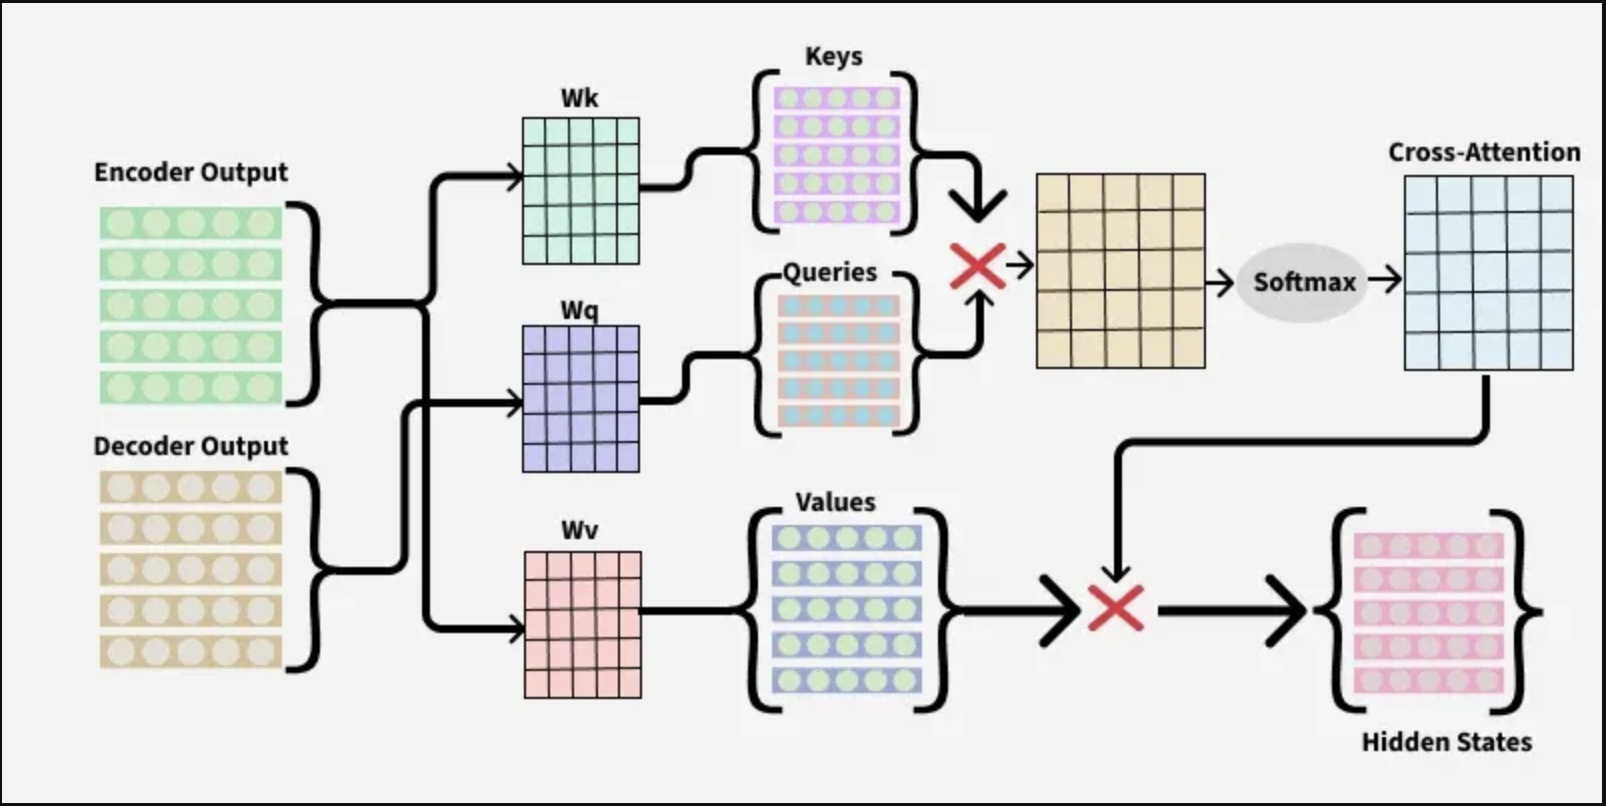
\includegraphics[width=1.2\linewidth]{f17.png}
        \renewcommand{\thefootnote}{}
        \footnotetext{image credit: www.geeksforgeeks.org/}

    \column{0.65\linewidth}
    \vspace{-1em}
    \begin{itemize}
        \item Query (Question): Decoder creates a "query".
        \item Keys and Values (Answers): Encoder provides "keys" and "values." 
        \item Matching: Cross-attention mechanism compares the query from the decoder with the keys from the encoder. 
    \end{itemize}
\end{columns}

\begin{itemize}
    \item Combining Information: The cross-attention mechanism combines the relevant information from the encoder (values) to help the decoder generate the next word in the translation.
\end{itemize}
\end{frame}

\begin{frame}{Inference Visualization}

\begin{figure}\renewcommand{\thefootnote}{}
\footnotetext{image credit: Shah Jainam}
    \centering
    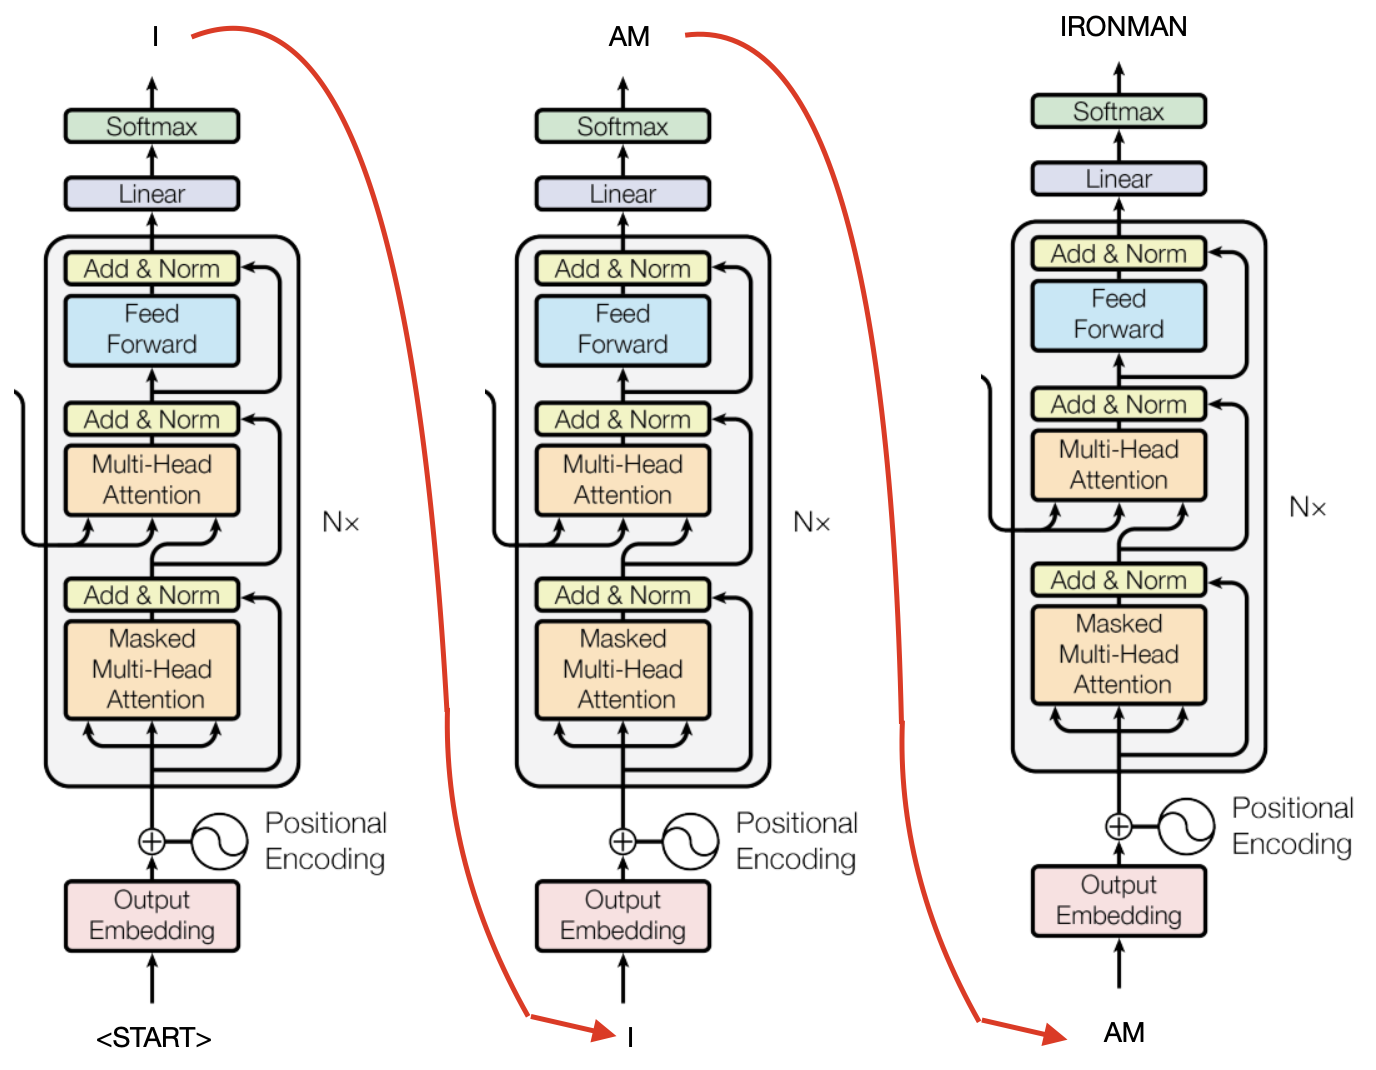
\includegraphics[width=0.8\linewidth]{f18.png}
    \label{fig:enter-label}
\end{figure}
    
\end{frame}

\begin{frame}{Why Self-Attention?}

Three criteria for consideration:
\begin{itemize}
    \item The total computational complexity per layer. 
    \item The amount of computation that can be parallelized, as measured by the minimum number of sequential operations required.
    \item The path length between long-range dependencies in the network.
    \begin{itemize}
        \item The shorter these paths between any combination of positions in the input and output sequences, the easier it is to learn long-range dependencies \footnote{Sepp Hochreiter, Yoshua Bengio, Paolo Frasconi, and Jürgen Schmidhuber}.
    \end{itemize}
\end{itemize}

\begin{figure}[htbp]
    \centering
    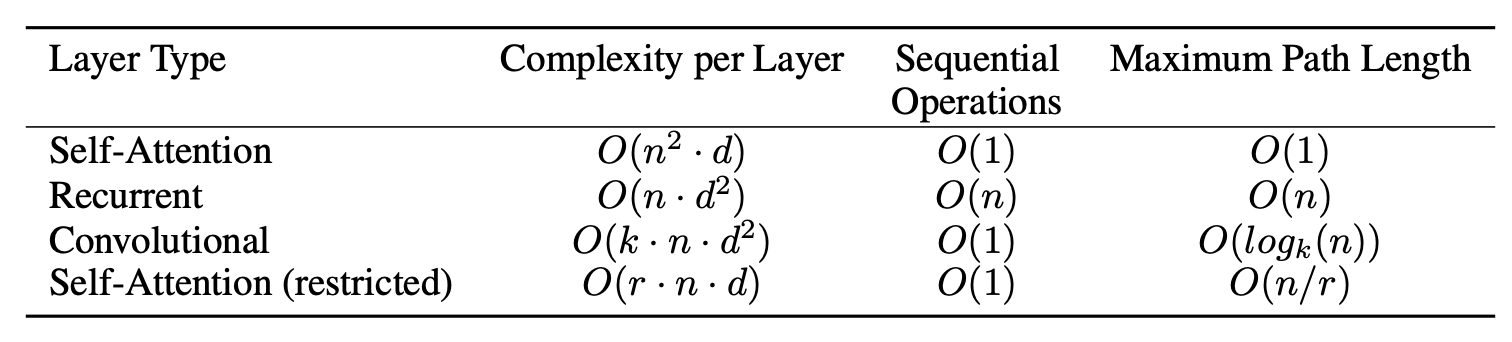
\includegraphics[width=1\linewidth]{f19.png}
    \label{fig:enter-label}
\end{figure}
\end{frame}

\begin{frame}{Complexity of layer types}

\begin{figure}\renewcommand{\thefootnote}{}
\footnotetext{image credit: Jeong-Gwan Lee}
    \centering
    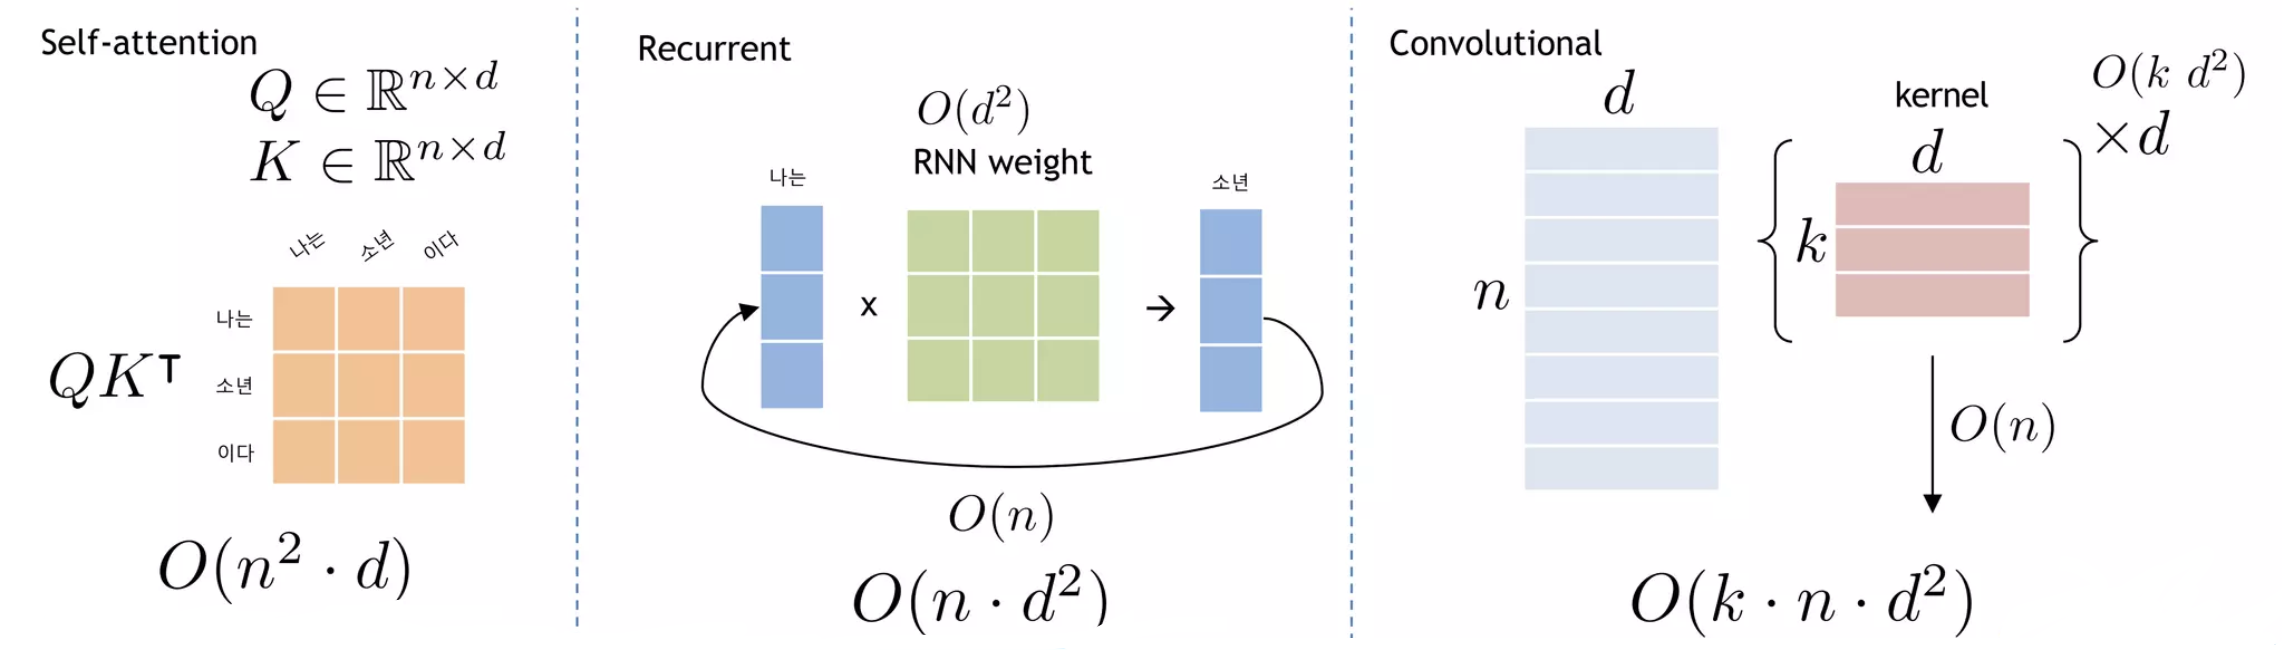
\includegraphics[width=0.7\linewidth]{f20.png}
    \label{fig:enter-label}
\end{figure}

\vspace{-1em}
\begin{itemize}
    \item Self-Attention
        \begin{itemize}
        \item Connectivity: All positions connected in constant sequential steps
        \item Parallelism: High; allows full parallel execution
    \end{itemize}
    
    \item Recurrent Layers (RNNs)
        \begin{itemize}
        \item Parallelism: Low; inherently sequential
        \item Complexity: Higher latency due to step-by-step processing
    \end{itemize}

    \item Convolutional Layers
        \begin{itemize}
        \item Kernel width $k<n$ $\rightarrow$ limited direct connectivity.
        \item Longer path lengths between distant positions
    \end{itemize}
\end{itemize}    
\end{frame}

\begin{frame}{Training}

\textbf{English-to-German: State-of-the-Art}
\begin{itemize}
  \item Transformer (Big) achieves \textbf{28.4 BLEU}
  \item Outperforms all previous models and ensembles by \textbf{+2.0 BLEU}
  \item Trained in \textbf{3.5 days on 8× P100 GPUs}
  \item Base Transformer also surpasses prior models at a lower training cost
\end{itemize}

\textbf{English-to-French: High Performance, Low Cost}
\begin{itemize}
  \item Transformer (Big) achieves \textbf{41.0 BLEU}
  \item Outperforms all previous single models
  \item Training cost is less than \textbf{¼ of previous state-of-the-art}
  \item Dropout used: $P_{drop} = 0.1$ (vs 0.3)
\end{itemize}

\textbf{Training \& Inference Details}
\begin{itemize}
  \item Checkpoint averaging:
    \begin{itemize}
      \item Base: last 5 checkpoints
      \item Big: last 20 checkpoints
    \end{itemize}
  \item Beam search: beam size = 4, length penalty $\alpha = 0.6$
  \item Output length: input length + 50 (early stopping enabled)
\end{itemize}

\textbf{Training Cost Estimation}
\begin{itemize}
  \item Estimated FLOPs = training time × \#GPUs × GPU FLOP capacity
\end{itemize}
    
\end{frame}

\begin{frame}{Model Comparisons}

The Transformer achieves better BLEU scores than previous state-of-the-art models on the
English-to-German and English-to-French newstest2014 tests at a fraction of the training cost. 

\begin{figure}[htbp]
    \centering
    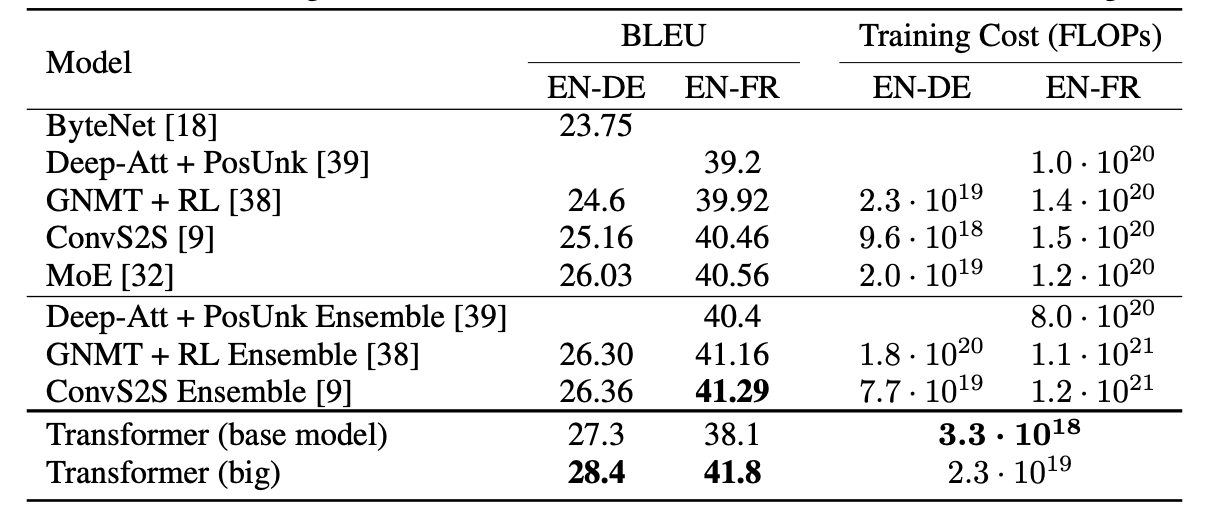
\includegraphics[width=1\linewidth]{f21.png}
    \label{fig:enter-label}
\end{figure}
    
\end{frame}

\begin{frame}{Model Variations}

Variations on the Transformer architecture. Unlisted values are identical to those of the base model. All metrics are on the English-to-German translation development set, newstest2013. Listed perplexities are per-wordpiece, according to our byte-pair encoding, and should not be compared to per-word perplexities
\begin{figure}
    \centering
    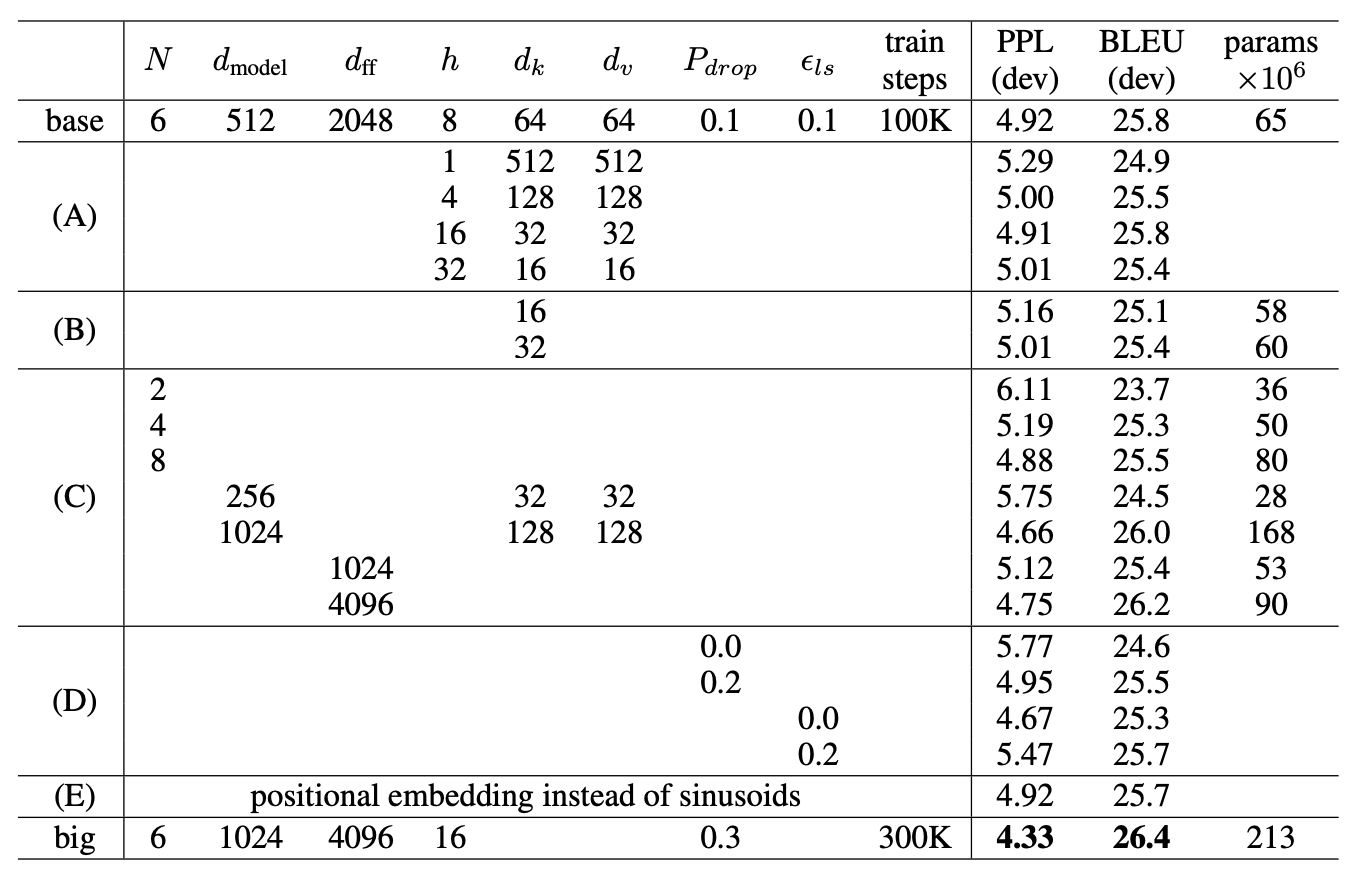
\includegraphics[width=0.75\linewidth]{f22.png}
    \label{fig:enter-label}
\end{figure}
\end{frame}

\begin{frame}{English Constituency Parsing}
\begin{itemize}
    \item To evaluate if the Transformer can generalize to other tasks, experiments on English constituency parsing.
    
    \item This task presents specific challenges: the output is subject to strong structural constraints and is significantly longer than the input. 
    
    \item Furthermore, RNN sequence-to-sequence models have not been able to attain state-of-the-art results in small-data regimes.
\end{itemize}

\begin{figure}
    \centering
    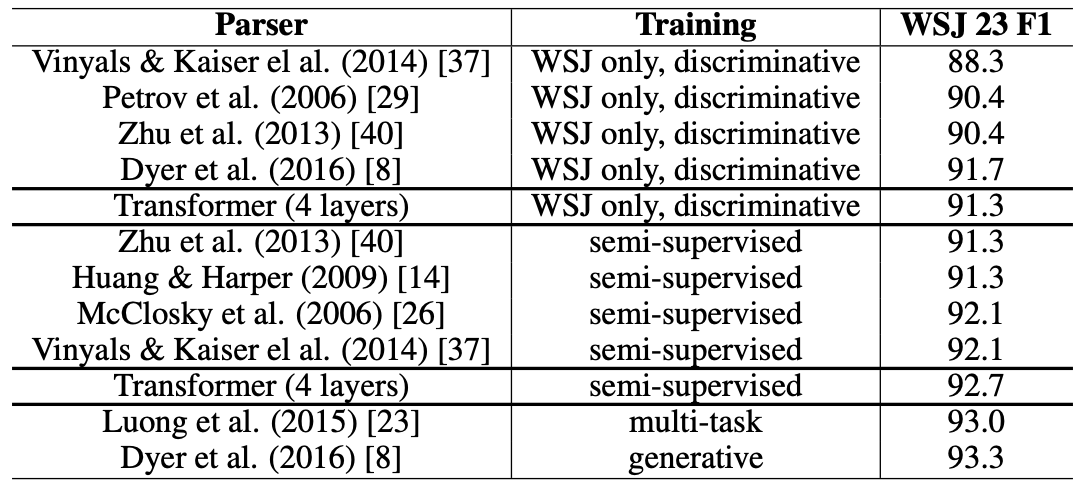
\includegraphics[width=0.8\linewidth]{f23.png}
    \label{fig:enter-label}
\end{figure}
\end{frame}

\begin{frame}{Limitations of Transformer}\renewcommand{\thefootnote}{}
\footnotetext{Angela Fan†
, Thibaut Lavril, Edouard Grave, Armand Joulin, Sainbayar Sukhbaatar}
\textbf{1. Walking Down a Corridor}
\begin{itemize}
    \item Agent sees a colored object (blue/green), walks a long corridor, and selects the correct colored door.
    \item \textbf{Result:} Transformer performance degrades with smaller memory.
\end{itemize}

\textbf{2. Copy and Reverse}
\begin{itemize}
    \item Input: Sequence of digits (0–9), length 40 (train), 400 (test).
    \item \textbf{Result:} Feedback Transformer shows large gains in accuracy and generalization.
\end{itemize}

\textbf{3. Counting}
\begin{itemize}
    \item Input: A’s repeated; Output: same number of B’s.
    \item \textbf{Result:} Feedback Transformer significantly better, especially on longer sequences.
\end{itemize}
    
\end{frame}

\begin{frame}{Future Works}




    
\end{frame}
    
\end{document}


